\documentclass{standalone}
\usepackage{tikz}
\begin{document}
    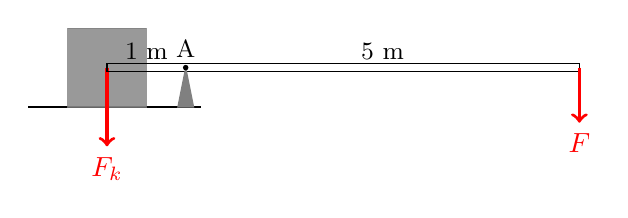
\begin{tikzpicture}
        % gólf
        \draw (-1,-0.5) -- (1.2,-0.5);
        % kassi
        \draw [fill=gray, color=gray, opacity=0.8] (-0.5,-0.5) rectangle (0.5,0.5);
        % kraftar
        \draw [very thick, ->,red] (0,0) -- (0,-1) node [below] {$F_k$};
        \draw [] (0,-0.05) rectangle (6,0.05);
        \draw [color=gray, fill=gray] (1,0)--(1.1,-0.5)--(0.9,-0.5) -- (1,0);
        \draw [very thick, ->,red] (6,0) -- (6,-0.7) node [below] {$F$};
        \fill (1,0) circle (1pt);
        \draw (1,0) node[above]{\small A};
        \draw (0.5,0.2) node[]{\small 1 m};
        \draw (3.5,0.2) node[]{\small 5 m};
    \end{tikzpicture}
\end{document}
